\documentclass[sigconf]{acmart}

\usepackage{booktabs} % For formal tables
\usepackage{hyperref}
\usepackage[l2tabu,orthodox]{nag}
\usepackage[utf8x]{inputenc}
\usepackage[british]{babel}
%\usepackage[babel=true]{microtype}
%\usepackage{amsmath}
%\usepackage[all]{onlyamsmath}
%\usepackage{newtxtext}
%\usepackage{newtxmath}
\usepackage{upquote}
\usepackage{graphicx}
\usepackage{url}
\usepackage{subfigure}
\usepackage{booktabs}
%\usepackage{bytefield}
%\usepackage{listings}
%\usepackage{algorithm}
%\usepackage{algpseudocode}
\usepackage{color}
\usepackage{balance}
\usepackage{tabularx}
%\usepackage{rotating}
%\usepackage{mathtools}
\usepackage{makecell}
\usepackage{subfigure}
\usepackage{amsmath}
\usepackage{algorithm}
\usepackage[noend]{algpseudocode}
% Copyright
%\setcopyright{none}
%\setcopyright{acmcopyright}
%\setcopyright{acmlicensed}
\setcopyright{rightsretained}
%\setcopyright{usgov}
%\setcopyright{usgovmixed}
%\setcopyright{cagov}
%\setcopyright{cagovmixed}
\newcommand{\todo}[1]{\textbf{\textcolor{red}{To do -- #1}}}
\graphicspath{{../figures/}}

% FIXME: correct \acmDOI{} and \acmISBN{} for camera ready, if accepted
\acmDOI{10.475/123_4}
\acmISBN{123-4567-24-567/08/06}

\acmConference[MMSys 2018]{ACM Multimedia Systems Conference}{June 2018}{Amsterdam, The Netherlands}
\acmYear{2018}
\copyrightyear{2017}
\acmArticle{4}
\acmPrice{15.00}
\begin{document}

\title{DASHing through Hollywood}

%\titlenote{Produces the permission block, and
%  copyright information}
%\subtitle{Extended Abstract}
%\subtitlenote{The full version of the author's guide is available as
%  \texttt{acmart.pdf} document}

% FIXME: add authors for camera ready, if accepted
\author{Anonymous}
%\orcid{1234-5678-9012}
\affiliation{%
  \institution{\ }
  \department{\ }
  \city{\ }
  \postcode{\ }
  \country{\ }
}
\email{anonymous@example.com}

% FIXME: add short authors for camera ready, if accepted
\renewcommand{\shortauthors}{Anonymous}


\begin{abstract}
Adaptive streaming over HTTP has become the de-facto standard for video streaming over the
Internet, partly due to its ease of deployment in a heavily ossified Internet. Though
performant in most on-demand scenarios, it is bound by the semantics of TCP, with
reliability prioritised over timeliness, even for live video where the reverse may be
desired. In this paper, we present an implementation of MPEG-DASH over TCP Hollywood, a
widely deployable TCP variant for latency sensitive applications. Out-of-order delivery
in TCP Hollywood allows the client to measure, adapt and request the
next video chunk even when the current one is only partially downloaded. Furthermore, the
ability to skip frames, enabled by multi-streaming and out-of-order delivery, adds resilience against stalling 
for any delayed messages. We observed
that in high latency and high loss networks, TCP Hollywood significantly
lowers the possibility of stall events and also supports better quality downloads in
comparison to standard TCP, with minimal changes to current adaptation algorithms. 
\end{abstract}

%
% The code below should be generated by the tool at
% http://dl.acm.org/ccs.cfm
% Please copy and paste the code instead of the example below. 
%
%\begin{CCSXML}
%<ccs2012>
% <concept>
%  <concept_id>10010520.10010553.10010562</concept_id>
%  <concept_desc>Computer systems organization~Embedded systems</concept_desc>
%  <concept_significance>500</concept_significance>
% </concept>
% <concept>
%  <concept_id>10010520.10010575.10010755</concept_id>
%  <concept_desc>Computer systems organization~Redundancy</concept_desc>
%  <concept_significance>300</concept_significance>
% </concept>
% <concept>
%  <concept_id>10010520.10010553.10010554</concept_id>
%  <concept_desc>Computer systems organization~Robotics</concept_desc>
%  <concept_significance>100</concept_significance>
% </concept>
% <concept>
%  <concept_id>10003033.10003083.10003095</concept_id>
%  <concept_desc>Networks~Network reliability</concept_desc>
%  <concept_significance>100</concept_significance>
% </concept>
%</ccs2012>  
%\end{CCSXML}
%
%\ccsdesc[500]{Computer systems organization~Embedded systems}
%\ccsdesc[300]{Computer systems organization~Redundancy}
%\ccsdesc{Computer systems organization~Robotics}
%\ccsdesc[100]{Networks~Network reliability}
%
%
%\keywords{ACM proceedings, \LaTeX, text tagging}


\maketitle

\section{Introduction}

% High-level: Internet video is significant, HAS protocols are a large part of that, but
% TCP isn't optimal

Video has grown to be the dominant class of traffic on the Internet in recent
years, and it is expected to grow further. This growth has been driven by a rising number
of cord-cutters: users who have switched to consuming video solely over the Internet. HTTP
Adaptive Streaming (HAS) protocols, including proprietary protocols such as Apple's HTTP Live
Streaming (HLS) and the MPEG-DASH standard, underpin much of this traffic.  HTTP uses TCP
at the transport-layer, however, which is suboptimal for applications that wish to trade-off
reliability and order for timeliness, including Internet video applications.

% Narrow down: what's our problem with standard MPEG-DASH over HTTP+TCP?

HAS protocols operate on a pull-based technique, driven by the client application. An HTTP
server provides video in discrete chunks of equal duration. Each chunk is provided in several 
different encodings, each at a different bit-rate. The client requests each chunk in turn, 
determining the
appropriate representation to request based on its rate adaptation algorithm. The client
then plays out these chunks in order, using a buffer to attempt to reduce stalling
behaviour when a chunk doesn't finish downloading in time to play. However, the application 
is bound by the reliable delivery
semantics of TCP: the application \emph{must} wait for undelivered chunks. Stalling for
undelivered chunks affects quality-of-experience, not only with the stall itself, but with
the signals that the delay provides to the rate adaptation algorithms. Transient network
issues are amplified.

% Contributions: what are we going to do/show?

In this paper, we develop an MPEG-DASH system that uses TCP Hollywood
\cite{mcquistin2016tcp,mcquistin2016tcp2}, a variant of TCP
that provides an unordered, multi-streaming delivery model. The changes made in
TCP Hollywood are intended to reduce the impact of
losses on quality-of-experience in high-delay networks. In high-delay and high-loss networks, 
adopting it for HAS results in total stall duration that is seven times lower than that of 
standard TCP.
Further, we show small improvements in start-up delay and average media bit-rate.

% What about other methods? Multiple HTTP/1.1 connections? HTTP/2?

Similar results could be achieved by using multiple simultaneous transport-layer
connections. However, these connections maintain separate flow and congestion control
states, resulting in degraded performance. Multi-streaming in HTTP/2 allows a single
transport-layer connection to be used by multiple ordered streams. Sending each chunk
within its own stream would remove application-layer head-of-line blocking, but not the
head-of-line blocking introduced by TCP. Our approach allows for a single transport-layer
connection to be used, with the benefits that come with this, while eliminating
head-of-line blocking.

% Paper structure

The remainder of this paper is structured as follows. Section \ref{sec:hlywd} briefly
introduces TCP Hollywood, and how its delivery semantics are useful for our application.
Section \ref{sec:transport} describes the changes required to our MPEG-DASH client and
server to work across TCP Hollywood. The testbed environment is described in Section
\ref{sec:methodology}, and the evaluation results are discussed in Section \ref{sec:testing}.
Finally, Section \ref{sec:related} discusses related work, and how our contribution fits
with this, while Section \ref{sec:conclusion} concludes.

\section{TCP Hollywood}
\label{sec:hlywd}

TCP Hollywood \cite{mcquistin2016tcp, mcquistin2016tcp2} is an unordered and time-lined
transport protocol. While maintaining wire compatibility with standard TCP, TCP Hollywood
removes two sources of transport-layer latency: in-order delivery and reliability.
In-order delivery results in head-of-line blocking: data is not made available to the
application until all earlier data has been delivered. Providing reliability over a
best-effort network requires retransmissions, adding latency while loss is detected and
retransmissions are sent. TCP Hollywood uses message-oriented semantics, and eliminates
head-of-line blocking by delivering messages to the receiver in the order that they
arrive. TCP Hollywood also relaxes standard TCP's reliability guarantee, providing
\emph{partial} reliability instead. The TCP Hollywood API allows applications to specify a
deadline for each message, after which it will no longer be sent -- this means that if a
retransmission of a lost message is unlikely to arrive before its deadline, it will not be
sent; an unexpired message will be sent instead (i.e., the retransmitted TCP segment's
payload is different to the original transmission). Making use of this functionality
requires that the application be aware of the TCP Hollywood extensions and the content
being sent, such that it can set a deadline for each message.

Under standard MPEG-DASH, when a frame is to be played out, but has not yet arrived, the
application will stall waiting for the missing data to arrive. When using standard TCP,
this is a sensible design choice: subsequent frames are not in the application buffer
either. However, when TCP Hollywood is used, and head-of-line blocking is eliminated,
later frames may be available to the application. This makes skipping frames a viable
design choice -- rather than waiting for the missing frame, it is better to use error
concealment techniques to minimise the impact of loss as much as possible and continue
play-back. Deeper analysis of TCP Hollywood \cite{mcquistin2016tcp, mcquistin2016tcp2},
which explores the impact of removing head-of-line blocking on application performance,
has been carried out.

The scope of this work is to evaluate the impact of HAS-over-TCP Hollywood on video
quality-of-experience, while minimising change at the application-layer (i.e., maintaining
alignment with the MPEG-DASH standard). One of the core tenets of the MPEG-DASH
architecture is that the application logic is driven by the client: it determines when,
and at which rate, chunks are requested. This means that the server can be a generic HTTP
server -- much of MPEG-DASH's popularity is owed to this approach. Given that TCP
Hollywood's deadline API requires state to be held at the server, we only consider the
benefits of its unordered delivery feature in this paper. 
\section{Unordered Delivery in MPEG-DASH}
\label{sec:transport}

MPEG-DASH is designed for an ordered transport protocol. Adapting it for an
unordered transport protocol requires several considerations. These
changes happen in two broad areas: the HTTP request and response semantics, and the rate
adaptation algorithms. We consider both of these in turn below.

\subsection{HTTP Request/Response Semantics}

TCP Hollywood operates on a message level and thus the decision to keep or discard is made
for a message. The application must therefore decide what each message should contain. In
the case of our HAS application, messages could contain either (i) an entire chunk of video; 
(ii) a video frame from within the chunk; or (iii) a fixed-sized message from within the 
chunk boundaries.  Sending an entire chunk as a TCP Hollywood
message means that the loss of a single TCP segment carrying part of that message could result in
the entire message being lost if it failed to be delivered before its deadline. Sending 
individual video frames would require the HTTP server to be content-aware, and able to 
split video chunks into frame; this is beyond the scope of our work given our goal of
maintaining alignment with the MPEG-DASH standard. Accordingly, we opt to send fixed-size 
messages (of 1400 bytes), which balances the impact of segment loss with being content-agnostic. 
The terminology and its use within the paper is further clarified in Figure \ref{fig:terminology}.

\begin{figure}
  \centering
  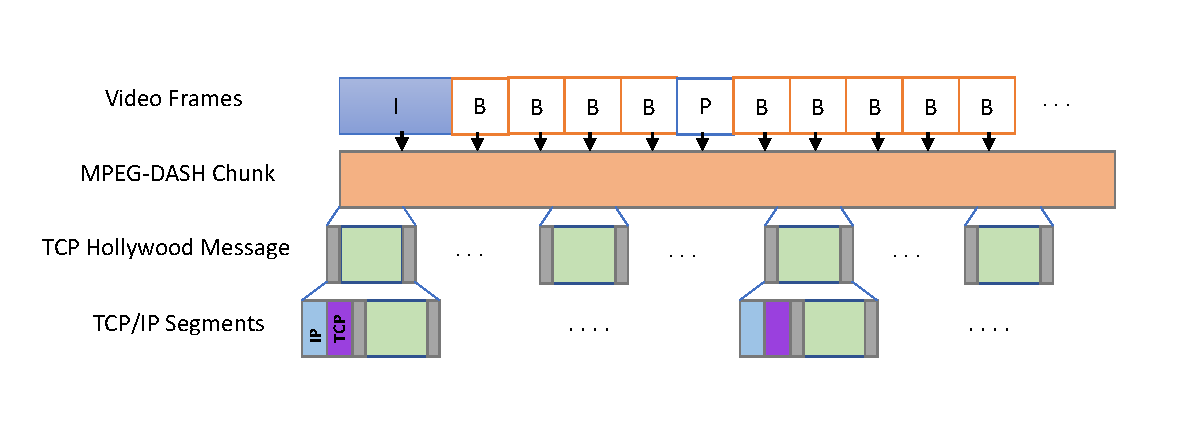
\includegraphics[width=\columnwidth]{figures/terminology2.pdf}
  \caption{Illustration of the terminology used in this paper and also the encapsulation of data for transport.}
  \label{fig:terminology}
\end{figure}

TCP Hollywood supports multi-streaming over a single TCP connection, allowing for the
separation of the control and data channels. We use separate streams for HTTP request and
response headers, sending each as separate TCP Hollywood messages. This allows the client
to request later chunks while earlier chunks are still downloading. The server still sends
chunks sequentially, but does not have to wait for the next request to arrive; this is
especially useful in high latency networks. Figure \ref{fig:hollywood_download}
illustrates chunk retrieval with HTTP over both standard TCP and TCP Hollywood.

Our use of multi-streaming in TCP Hollywood is similar to HTTP/1.1 pipelining and bundle
requests in HLS \cite{muller2012evaluation}. However, these approaches require quality
estimates to be submitted for all chunks at request time. This means that a quality
estimate may be two or more chunk durations old before being used at the server.
Fluctuations in network conditions in the interval between request and response mean that
these quality estimates can be incorrect. Under TCP Hollywood, requests can be sent while
chunks are downloading, allowing for the server to receive a more recent and accurate
estimate of network conditions. This reduces the likelihood of an under or over estimation
of performance, improving quality-of-experience. Further, HTTP/1.1 pipelining suffers
from transport-layer head-of-line blocking in standard TCP, which is eliminated under TCP Hollywood.

Finally, TCP Hollywood can discard late messages and continue play-out,
thereby limiting stall events only to those cases when the play-out buffer is completely
empty.

\begin{figure}
    \centering
    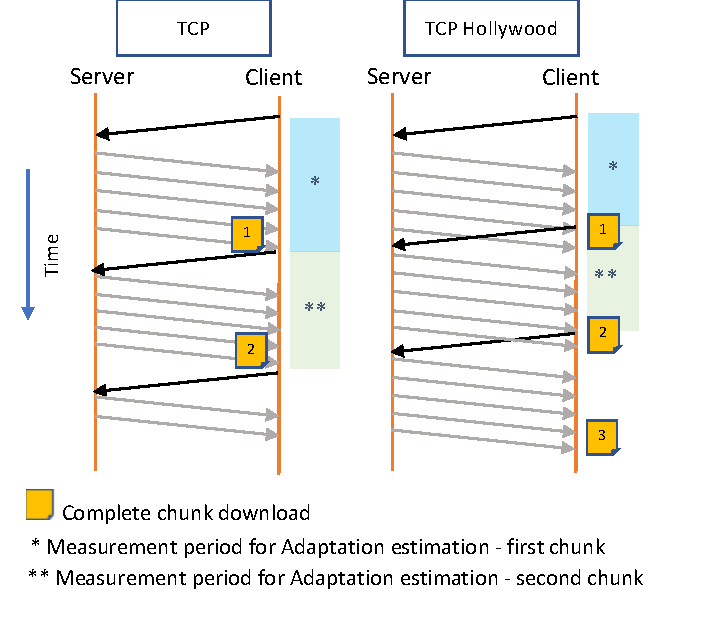
\includegraphics[width=\columnwidth]{figures/tcph-download.pdf}
    \caption{An illustration of chunk download with HTTP over TCP and over TCP Hollywood. The measurement period for first chunk is shown in blue while that of the second chunk is shown in green. }
    \label{fig:hollywood_download}
\end{figure}

The requested chunks of video are transmitted on a single stream, using fixed size
messages. As the server is content-agnostic, it is unable to set an expiry time for messages, and
all messages are sent reliably. A content-aware server would set this to the relative presentation time of the chunk.
For the sake of simplicity, audio
stream is not used. Each message is appended with a monotonically increasing sequence
number and a stream offset. The stream offset is the offset of the last byte of the
message within this stream, where a stream includes all chunks that have been transmitted
previously. Both fields are used by the receiver to reorder the messages and detect
losses. We expanded the function of the play-out buffer to include de-jittering and
reordering of the incoming messages.

% FIXME: explain why MP4 is not suitable [csp]
It is also important to use a media format that is tolerant of packet losses. Hence, the
commonly used ISO Base Media File Format (MP4) is not suitable for TCP Hollywood, so we
use MPEG Transport streams (TS) instead. The use of MPEG-TS streams is allowed as part of
the MPEG-DASH standard and are also used by HLS.

\subsection{Rate Adaptation Algorithms}

Performance of a MPEG-DASH system relies heavily on a good rate adaptation algorithm.
Such algorithms use application-level measurements such as buffer length, throughput, time to
download a chunk, or a combination of these to select an appropriate quality for
download \cite{beben2016abma+, spiteri2016bola, li2014probe}. There is some consensus
among researchers that buffer-based algorithms are more performant and reliable in a wider
variety of network conditions than other algorithms 
\cite{huang2015buffer, karagkioules2017comparative}.

Our TCP Hollywood-based MPEG-DASH client uses a modified version of the open-source BOLA 
(Buffer Occupancy based Lyapunov Algorithm) rate adaptation algorithm \cite{spiteri2016bola}. 
BOLA is part of the MPEG-DASH reference
client, dash.js.\footnote{\url{https://github.com/Dash-Industry-Forum/dash.js/wiki}}
BOLA uses the amount of video currently buffered to calculate the quality level (bit-rate
level) for the next chunk. For live video, where buffer sizes are limited, the algorithm
uses throughput estimates to further reduce over-estimation and stalling. In the presence
of packet loss and duplication, that is possible with TCP Hollywood, the calculation 
mechanisms for both measurements have to be modified. For a standard MPEG-DASH client,
the HTTP request for the next chunk is always sent 
during the download of the current chunk. For our TCP Hollywood-based client, we
introduce a new parameter, $Rx_{T}$, the receive ratio threshold. We modify
the rate adaptation algorithm so that if $Rx_{T}$ of the
bytes from a chunk have been received and the buffer is not filled to capacity, 
it estimates the quality of the next chunk based on the \emph{current} measurements and
sends a GET request to the server. Throughput is measured from the time the HTTP response
of a chunk arrives until $Rx_{T}$ is reached, excluding any duplicates. We experimented
with different values of $Rx_{T}$ and found 0.9 to be a suitable ratio. The full duration
of the chunk is used when calculating the buffer level, even though the entire chunk has
not been downloaded. With an $Rx_{T}$ value of 0.9, this is a safe assumption: only 10\%
of the chunk remains to be downloaded, with some data in-flight, and a limited number of
messages that may delayed (and subsequently discarded by TCP Hollywood if
they miss their deadline).
% FIXME: probably outside the scope of the initial submission, but it would
% be appropriate to describe the experiments and results that led to the
% choice of 0.9 as a parameter [csp]

% FIXME: "uses an effective buffer level" to do what? [csp]
BOLA uses an effective buffer level in the event that the chunk download is slowed by
the availability of the next chunk at the server (e.g., it has not been captured yet, as
in live scenarios) or by the size of the play-out buffer. In this case, as the buffer level has not
been limited by network conditions, the client is able to request higher quality chunks.
Therefore, the effective buffer level is the current buffer level, plus the time spent
waiting before downloading the next chunk. With TCP Hollywood, messages may be discarded
due to late arrival. If the buffer contains more than one chunk, we reduce the length of
effective buffer level by one chunk duration.


\begin{algorithm}
\begin{algorithmic}[1]
\Procedure{DownloadStream}{}
\State $\textit{n} \gets \textit{index of current chunk}$
\State $N \gets \textit{Total number of chunks}$
\State $q \gets \textit{Quality of the chunk}$
\State ${InitializeMetrics()}$
\While {$\text{n} < \text{N}$}
\State ${q \gets RunAlgorithm()}$
\State ${DownloadChunk(q, n)}$
\State ${UpdateMetricsUsingLastDownload()}$
\EndWhile
\EndProcedure
\end{algorithmic}
\caption{DASH Client Operation with TCP}\label{euclid}
\end{algorithm}
 

\begin{algorithm}
\caption{DASH Client Operation with QUIC}\label{euclid}
\begin{algorithmic}[1]
\Procedure{DownloadStream}{}
\State $\textit{n} \gets \textit{index of current chunk}$
\State $N \gets \textit{Total number of chunks}$
\State $q \gets \textit{Quality of the chunk}$
\State $S_n^q \gets \textit{Size of chunk with index n and quality q}$
\State $B_n^q  \gets \textit{Bytes received for chunk with index n and quality q }$
\State $Rx_T \gets Minimum Receive Threshold$
\State ${InitializeMetrics()}$
\While {$\text{n} < \text{N}$}
\State ${q \gets RunAlgorithm()}$
\State $InitiateChunkDownload(q, n)$
\While {$B_n^q < Rx_T * S_n^q$}
\State $Wait()$
\EndWhile
\State ${UpdateMetricsUsingLastDownload()}$
\EndWhile
\EndProcedure
\end{algorithmic}
\end{algorithm}

The algorithm is as follows 

\begin{algorithm}
\caption{BOLA with TCP Hollywood}\label{euclid}
\begin{algorithmic}[1]
\Procedure{DownloadStream}{}
\State $\textit{n} \gets \textit{index of current chunk}$
\State $N \gets \textit{Total number of chunks}$
\State $B \gets \textit{Maximum Buffer Length}$
\State $b_{now} \gets \textit{Current Buffer Length}$
\State $b_{p} \gets \textit{PlaceHolder Buffer}$
\While {$\text{n} < \text{N}$}
\If {$b_{now} > B$}
\State $\Delta t \gets B - b_{now}$
\State $wait (\Delta t)$
\EndIf
\State ${b_{p} \gets b_{p} + \Delta t}$
\State ${q \gets GetBolaQualityEstimate(b_p, b_{now})}$
\While {$bytes_rx < Rx_T x size(n_q)$}
\EndWhile
\EndWhile
\EndProcedure
\end{algorithmic}
\end{algorithm}
=======


%
%For the latter, we use the parameter rxratio (Receive ratio); the receiver will stop
%actively receiving a chunk if it has already received rxratio times the total bytes in
%the chunk and move on to estimating quality and requesting the next chunk. Since we use a
%buffer based algorithm, we still assume that we have received the entire chunk while
%calculating the quality of the next chunk. Note that the remaining chunk is still being
%received passively, which means that the data is not used in throughput calculations for
%the adaptation algorithm. 
%

\section{Evaluation Methodology}
\label{sec:methodology}

We evaluate MPEG-DASH performance using both standard TCP and TCP Hollywood, to understand 
how the changes to the transport protocol affect quality of experience for streaming video.
Both standard TCP and TCP Hollywood use the CUBIC congestion control algorithm; both would
be impacted by any change to the variant of TCP used.

Our evaluation setup consists of a virtual environment that uses
Mininet\footnote{\url{https://mininet.org}} to create a virtual network with a modified
Linux kernel including the TCP Hollywood patches. We used our own MPEG-DASH server and client
implementation. The TCP Hollywood API was disabled when testing with standard TCP, and a
persistent HTTP/1.1 connection was used in both cases. The virtual network used included a single
client and server connected through a switch. Path characteristics were emulated at the
server interface using 
netem\footnote{\url{https://wiki.linuxfoundation.org/networking/netem}} Token Bucket
Filter traffic control, with a fixed 5Mbps line rate, a reasonable value for our test
videos, where the highest quality is 5600kbps. The test cases are divided into two
categories: (i) a loss rate of 0.2\% (random loss) with network latencies (RTT) between 150 to
400ms; and (ii) loss rates between 0 and 1\% with network latency of 100ms. Additional testing
was carried out with varying network conditions to evaluate adaptability.

\begin{table}[!t]
    \begin{tabular}{ccccc}
        \toprule
        \thead{Index} & \thead{Encoding bit-rate\\(kbps)} & \thead{Chunk bit-rate\\(kbps)} & \thead{PSNR} & \thead{SSIM} \\
        \midrule 
            1 & 1200 & 1301 & 37.220176 & 0.955177 \\
            2 & 1800 & 1941 & 39.142917 & 0.967720 \\
            3 & 2400 & 2584 & 40.478799 & 0.974580 \\
            4 & 3000 & 3228 & 41.515695 & 0.978962 \\
            5 & 3500 & 3766 & 42.226845 & 0.981527 \\
            6 & 4000 & 4304 & 42.845958 & 0.983509 \\
            7 & 5000 & 5328 & 43.868625 & 0.986314 \\
            8 & 5600 & 6030 & 44.387282 & 0.987527 \\
        \bottomrule
    \end{tabular}
    \caption{Video representations; all representations have a resolution of
             1920x1080p. PSNR and SSIM of re-encodings calculated against original Y4M reference.}
    \label{tab:testvideos}
\end{table}

We used Big Buck Bunny\footnote{\url{https://peach.blender.org}} with 8 quality levels as a video 
test sequence. The encoding bit-rates ranged from 1200 to 5600kbps with a constant resolution of 
1920x1080p. The constant resolution eliminates the need for re-scaling in objective Quality of 
Experience (QoE)
computations, which require the videos to be of the same resolution. MPEG-TS
are used to allow loss recovery. The use of MPEG-TS adds about a
10\% metadata overhead to the streams in our case (the use of MPEG-TS is not
essential to our approach, and any encoding or container format that is robust to packet loss
could be used). The encoding details for the different quality levels of
the test sequence are given in Table \ref{tab:testvideos}.
As TCP Hollywood is designed for low-latency applications, we use a 16 second buffer, with
a 1 second chunk duration.

To compare the performance of MPEG-DASH over standard TCP and TCP Hollywood, we use a number of 
Quality of Service (QoS) and QoE metrics: 
\begin{description}
    \item[Start-up delay] \hfill \\
        The amount of time from the start of the test until 2 seconds of video has been downloaded and demuxed.
    \item[Stall duration] \hfill \\
        The total amount of time the video stalls due to a completely empty buffer. The
        client would wait for one additional chunk to be downloaded before resuming play-out
        when a stall occurs.
    \item[Adaptability and stability] \hfill \\
        Adaptability is a measure of how quickly the adaptation algorithm can adapt to change in network conditions and stability is characterised by the client's ability to mitigate frequent bit rate fluctuations. These are measured using two metrics: (i) the average bit-rate of the downloaded chunks (adaptability), and (ii) the percentage of chunks with a downward bit-rate switch during play-out (stability).  
    \item[Objective QoE] \hfill \\
        To measure the level of distortion produced due to a discarded message, we use the 
        objective QoE metrics Peak Signal to Noise Ratio (PSNR) and Structural Similarity
        (SSIM). Both metrics are full-reference. We use the original Y4M sequence as
        reference and FFmpeg\footnote{\url{https://ffmpeg.org/ffmpeg-filters.html}} for the
        computation. Since PSNR and SSIM values will be lower for lower quality chunks, the
        metrics also provide a measure of quality even in the absence of discarded messages.
\end{description}

These metrics were chosen since they are widely used and have been shown to
be representative of different aspects of the user experience for MPEG-DASH
video.

\section{Results}
\label{sec:testing} 

In this section, we present the findings of our evaluation. All test cases were repeated
ten times and the depicted values are trimmed averages taken after discarding the highest
and lowest values. 
% FIXME: why this, rather than presenting error bars? [csp]

\subsection{Stall Events}
\label{sec:testing-stall}

The single most impactful impairment for DASH video user experience has been found to be
stall events \cite{hossfeld2011quantification}. A perfect adaptation algorithm would
eliminate stall events during video play-out by pre-buffering content and by adjusting the
download quality of the video to match the network performance. However, in reality, stall
events occur, due to imperfect estimates of network conditions.

As we might expect, TCP Hollywood offers most benefit in the presence of moderate losses and high
delay. Figure \ref{fig:stall_delay2} shows the effect of network latency on the total
stall duration experienced over standard TCP and TCP Hollywood when the line rate and loss
rate were kept constant at 5Mbps and 0.2\% respectively. At lower network latency, loss
recovery is quick and hence TCP Hollywood and standard TCP have similar performance.
However, for higher network latency, head-of-line blocking in standard TCP prevents data
that has already arrived from reaching the application. When the missing TCP segment does
arrive, the client can read a larger amount of data into its play-out buffer. On average,
no more than one or two TCP Hollywood messages are discarded at network latencies of 300ms and
350ms. The additional performance comes from the ability of the rate adaptation algorithm in 
our TCP Hollywood-based MPEG-DASH client to compute metrics and decide the quality of the 
next chunk before the delivery of the current chunk (see Section \ref{sec:transport}). 
This would mean that the client does not have to wait unnecessarily for the arrival of 
retransmissions before requesting the next chunk, helping to avoid stalls.

\begin{figure}
  \centering
  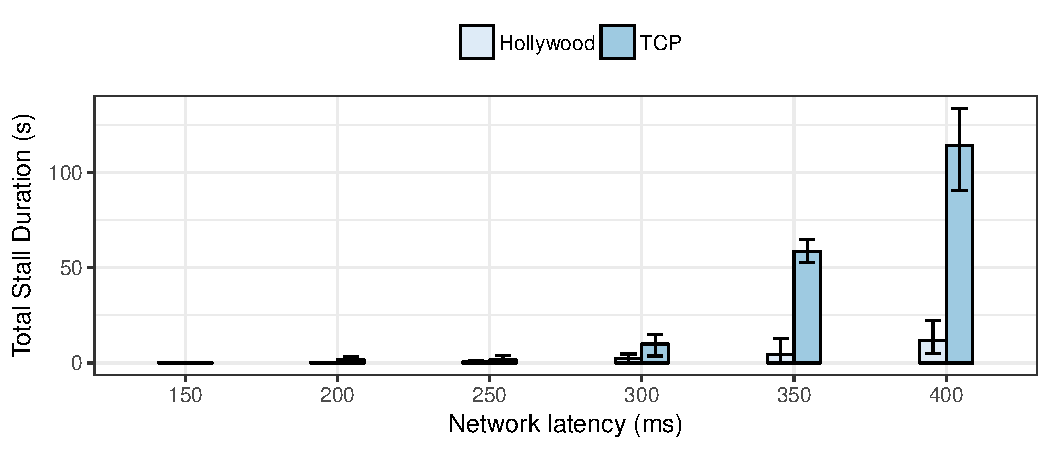
\includegraphics[width=\columnwidth]{figures/results/stall_sn_loss_p2.pdf}
  \caption{Stall events. Test networks were 5Mbps with 0.2\%loss with variable delay. The 
           client using standard TCP suffers more from stalls than the client using TCP Hollywood, 
           with the latter being able to minimise stalls in the presence of high network delay.}
  \label{fig:stall_delay2}
\end{figure}

\begin{figure}
  \centering
  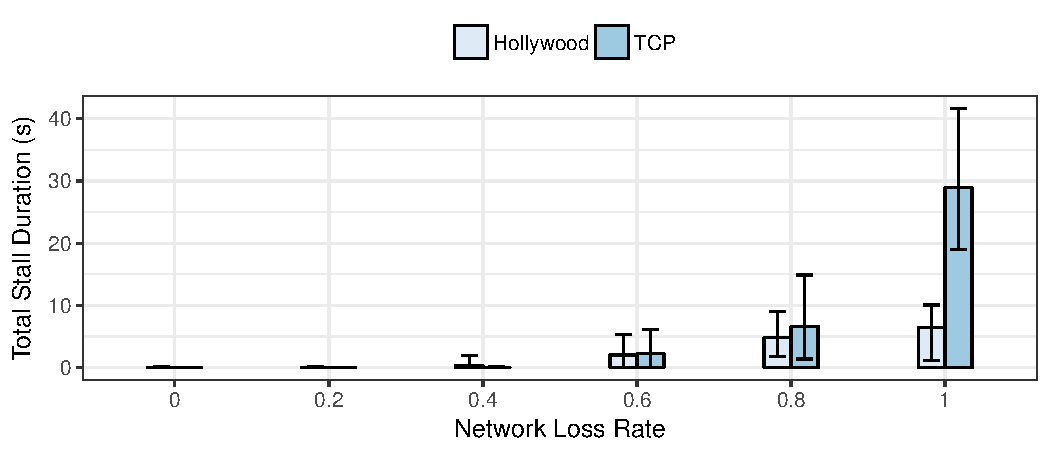
\includegraphics[width=\columnwidth]{figures/results/stall_sn_delay_d100.pdf}
  \caption{Stall events. Test networks were 5Mbps with 100ms with variable loss rates. With 
           high loss rates, loss recovery can be delayed due to lost retransmissions, leading 
           to more stall events for client using standard TCP.}
  \label{fig:stall_loss}
\end{figure}

When loss is high and delay is low, MPEG-DASH over TCP Hollywood and over standard TCP 
generally have similar performance. As packet loss increases, the TCP Hollywood-based 
client sees some performance benefit. Figure
\ref{fig:stall_loss} shows the results when network latency is 100ms, line rate is 5Mbps
and different network delays are used. When using loss rates of 0.6\% and 0.8\%, we
observed that the TCP Hollywood-based client is able to avoid some stall events by discarding 
some late arriving messages, however the benefit is very small in comparison to standard TCP 
as loss recovery is fast at low RTTs. At loss rates of 1\%, we observe that the advantage 
of using TCP Hollywood is significant, keeping the stall values for that client at around 5
seconds, in comparison with around 30 seconds in the case of the client using standard TCP 
for a 10 minute video. At high loss rates, the possibility of losing a retransmitted TCP 
segment become higher and loss recovery becomes a time consuming process even at lower 
network delays. 

\subsection{Start-up Delay}
We measure the start-up delay from the beginning of the test to the point when two seconds of
video (two chunks) have been downloaded and buffered, including the time taken to fetch the manifest
file. We use persistent connections for both standard TCP and TCP Hollywood, allowing the
TCP connection establishment and slow start latencies to be amortised across a longer
duration. In the case of TCP Hollywood, play-out can begin before the download of the
second chunk is complete, unlike standard TCP. However, as we use a receive ratio of 0.9,
the advantage is not significant for high speed networks. We still observe faster startup
values for TCP Hollywood in all scenarios because of its ability to request chunks
earlier. The higher the network latency, the greater the benefit of TCP Hollywood.

Figures \ref{fig:startup_delay2} and \ref{fig:startup_loss} show startup delay values
observed in our experiments. In the presence of higher losses, the startup delay can
become less stable and statistical significance in average values is lowered. For this
reason, the median value after eliminating the highest and the lowest observed values are
shown in the graphs.

\begin{figure}
  \centering
  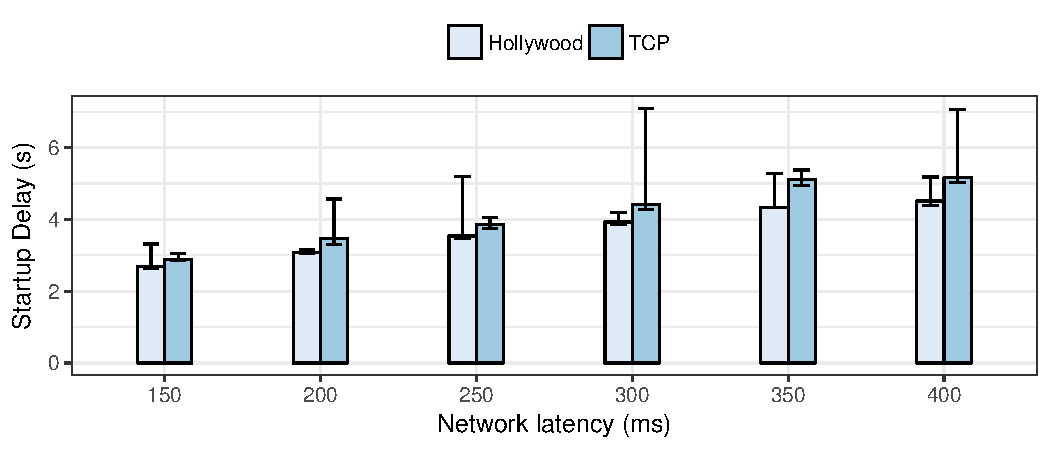
\includegraphics[width=\columnwidth]{figures/results/startup_sn_loss_p2.pdf}
  \caption{Start-up delay. Test networks were 5Mbps with 0.2\%loss with variable delay. 
           The higher the network latency, the greater the benefit of TCP Hollywood. }
  \label{fig:startup_delay2}
\end{figure}


\begin{figure}
  \centering
  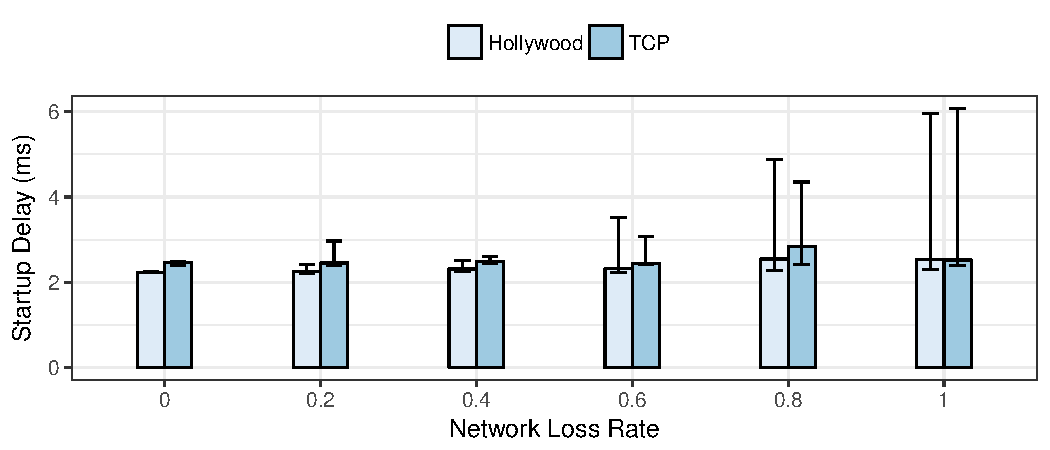
\includegraphics[width=\columnwidth]{figures/results/startup_sn_delay_d100.pdf}
  \caption{Start-up delay. Test networks were 5Mbps with 100ms with variable loss rates.  
           The start-up delay is slightly lower for the TCP Hollywood-based client.}
  \label{fig:startup_loss}
\end{figure}

\subsection{Adaptation and Stability}
While stall durations can be significantly reduced for high delay and high loss networks
by eliminating head-of-line blocking using TCP Hollywood, these improvements only hold
real significance if a TCP Hollywood-based client is able to deliver them while maintaining
the same level of video quality as a standard TCP-based client. Figure \ref{fig:rate_delay2} 
shows the effect of network latency on the average bit-rate of the video chunks for each transport
protocol. It can be seen that TCP Hollywood has a higher average bit-rate with a similar
level of standard deviation when network delay is 150ms and 200ms. For higher network
delay, TCP Hollywood continues to deliver chunks at a higher average bit-rate value than
standard TCP. In general, standard TCP appears to be more stable, as exhibited by the
percentage of chunks with a rate drop shown in Figure \ref{fig:ratechange_delay2}. A rate
drop is counted each time a chunk is downloaded at a bit-rate which is lower than the chunk
immediately before it. The difference in rate drops is equivalent to about 1 additional
drop observed per minute for TCP Hollywood than for standard TCP.

\begin{figure}
  \centering
  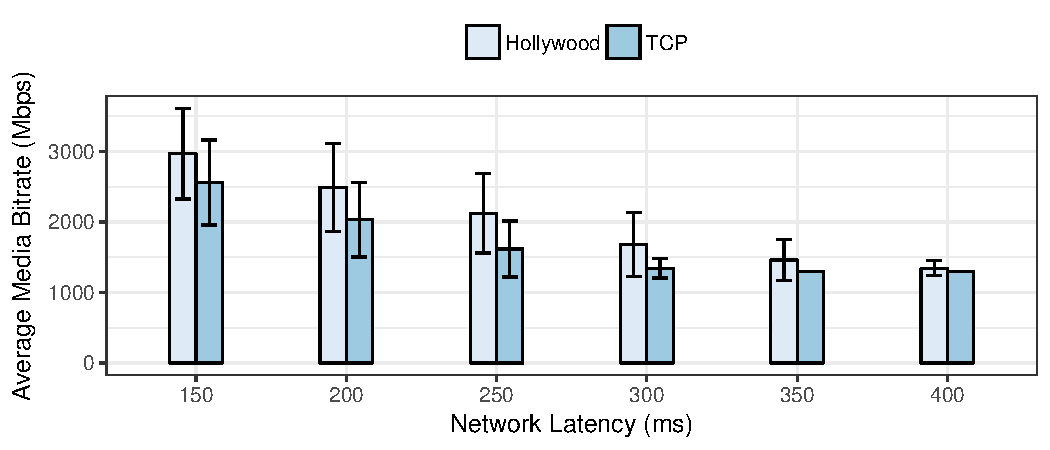
\includegraphics[width=\columnwidth]{figures/results/bitrate_sn_loss_p2.pdf}
  \caption{Adaptation and stability. Test networks were 5Mbps with 0.2\%loss with variable 
           delay. The error bars represent standard deviation. For higher delay values, 
           standard TCP shows lower standard deviation because it remains mostly at the 
           lowest available bit-rate. }
  \label{fig:rate_delay2}
\end{figure}

\begin{figure}
  \centering
  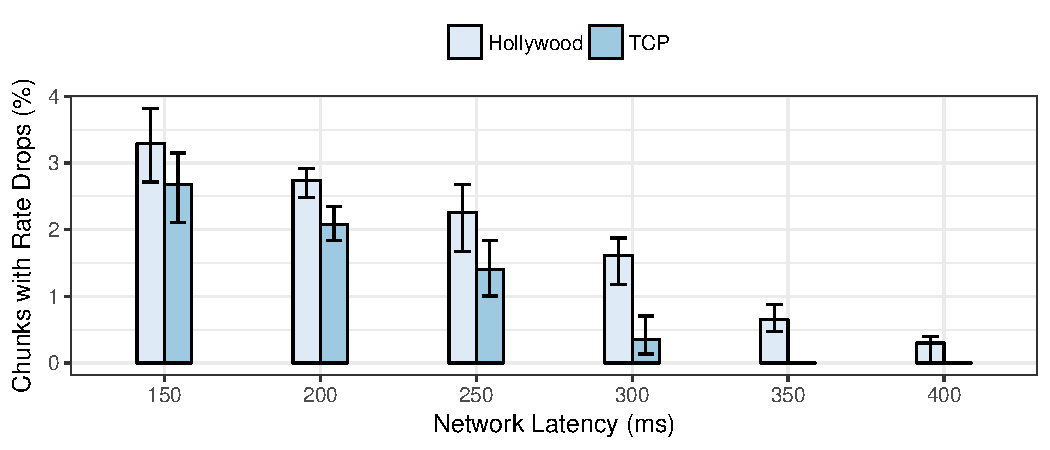
\includegraphics[width=\columnwidth]{figures/results/ratedrops_sn_loss_p2.pdf}
  \caption{Adaptation and stability. Test networks were 5Mbps with 0.2\%loss with variable 
           delay. The graph shows the percentage of chunks that were downloaded at a lower 
           rate than the previous one. The standard TCP adaptation algorithm is more stable 
           for all networks. The test video had 597 chunks.}
  \label{fig:ratechange_delay2}
\end{figure}

We observe that when packet loss is kept under 0.1\%, clients using both standard TCP and TCP 
Hollywood exhibit similar behaviour. As shown in Figure \ref{fig:rate_loss}, where network delay is 100ms, 
the TCP Hollywood-based client was able to deliver a higher average bit-rate than the standard TCP-based client, as
loss rates increased. Figure \ref{fig:ratechange_loss} shows the stability of the rate adaptation
stability under both standard TCP and TCP Hollywood. At a loss rate of 0.2\%, we found that the
TCP Hollywood-based client had higher stability than the standard TCP-based client. However,
for higher loss rate values, the TCP Hollywood-based client is less stable, as it attempts
to download higher bit-rate chunks, while the standard TCP-based client maintains stability
at the lowest bit-rate.

\begin{figure}
  \centering
  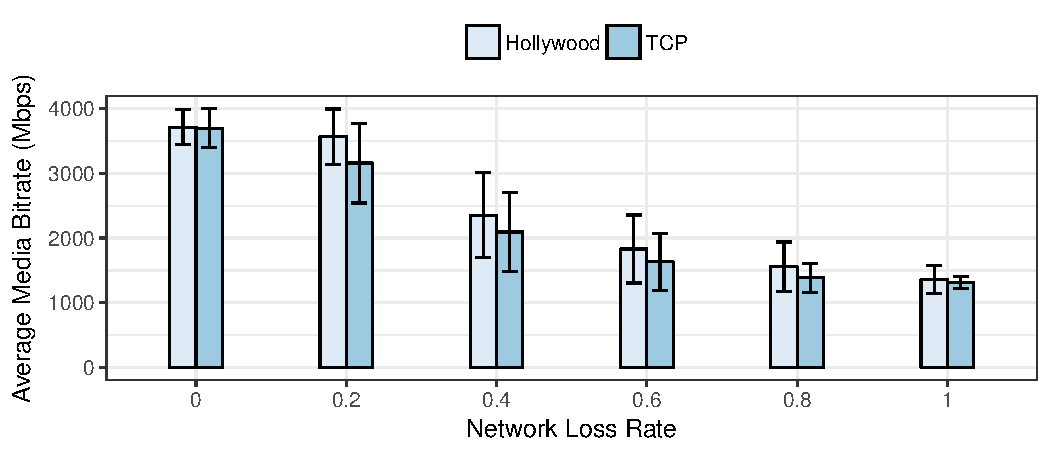
\includegraphics[width=\columnwidth]{figures/results/bitrate_sn_delay_d100.pdf}
  \caption{Test networks were 5Mbps with 100ms with variable loss rates. TCP Hollywood 
           significantly outperforms standard TCP at loss rate of 0.2\% with a higher 
           average rate and lower standard deviation. Error bars represent standard deviation.}
  \label{fig:rate_loss}
\end{figure}

\begin{figure}
  \centering
  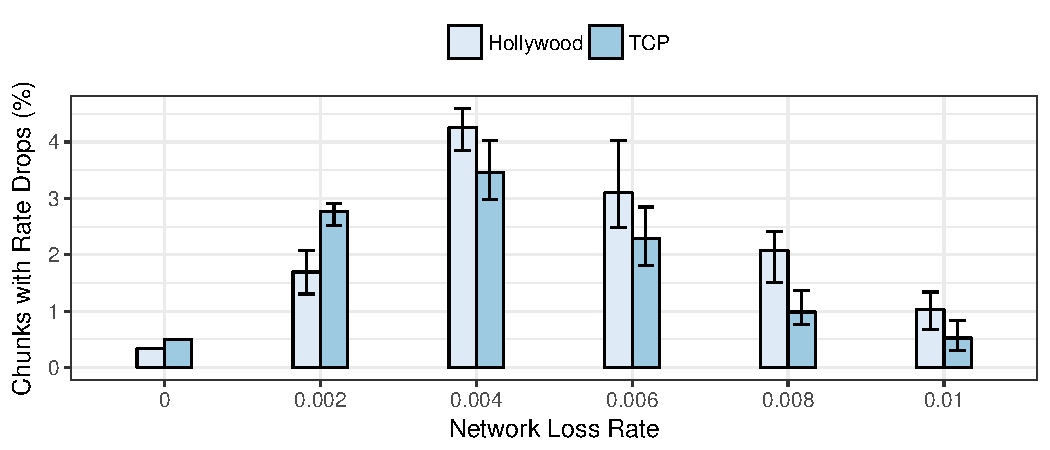
\includegraphics[width=\columnwidth]{figures/results/ratedrops_sn_delay_d100.pdf}
  \caption{Test networks were 5Mbps with 100ms with variable loss rates. Hollywood is more 
           stable for 0.2\% and no loss cases, however, at higher loss levels, standard TCP 
           becomes more stable.}
  \label{fig:ratechange_loss}
\end{figure}

\subsection{Quality of Experience}
None of the previously discussed metrics quantify the impact of the dropped messages
on a TCP Hollywood-based DASH client. A discarded message will result in visual impairments
that are not possible for a client using a reliable TCP stream. Figure \ref{fig:qoe_delay2} 
and \ref{fig:qoe_loss} show the observed PSNR and SSIM values of the received streams for the 
different transport options. The figures show box plots of frame-level PSNR and SSIM values 
observed during multiple
iterations of the test. Note that although the two objective QoE metrics represent the
quality of the chunks and the level of visual impairments due to discarded packets, it
does not show the impact of stall events, which were discussed in
Section \ref{sec:testing-stall}. Across all of the tests we ran in these experiments,
about 30\% of streams discarded at least one message during the 10 minutes of the video,
however, of these only 5\% lost more than 10 messages. Furthermore, the impact of a lost
message is most evident when a part of an I frame is lost. However, since chunks begin with
an I frame, the effect of even the worst visual impairment does not propagate farther than
the duration of the chunk, which in our case is 1 second.

\begin{figure}
  \centering
  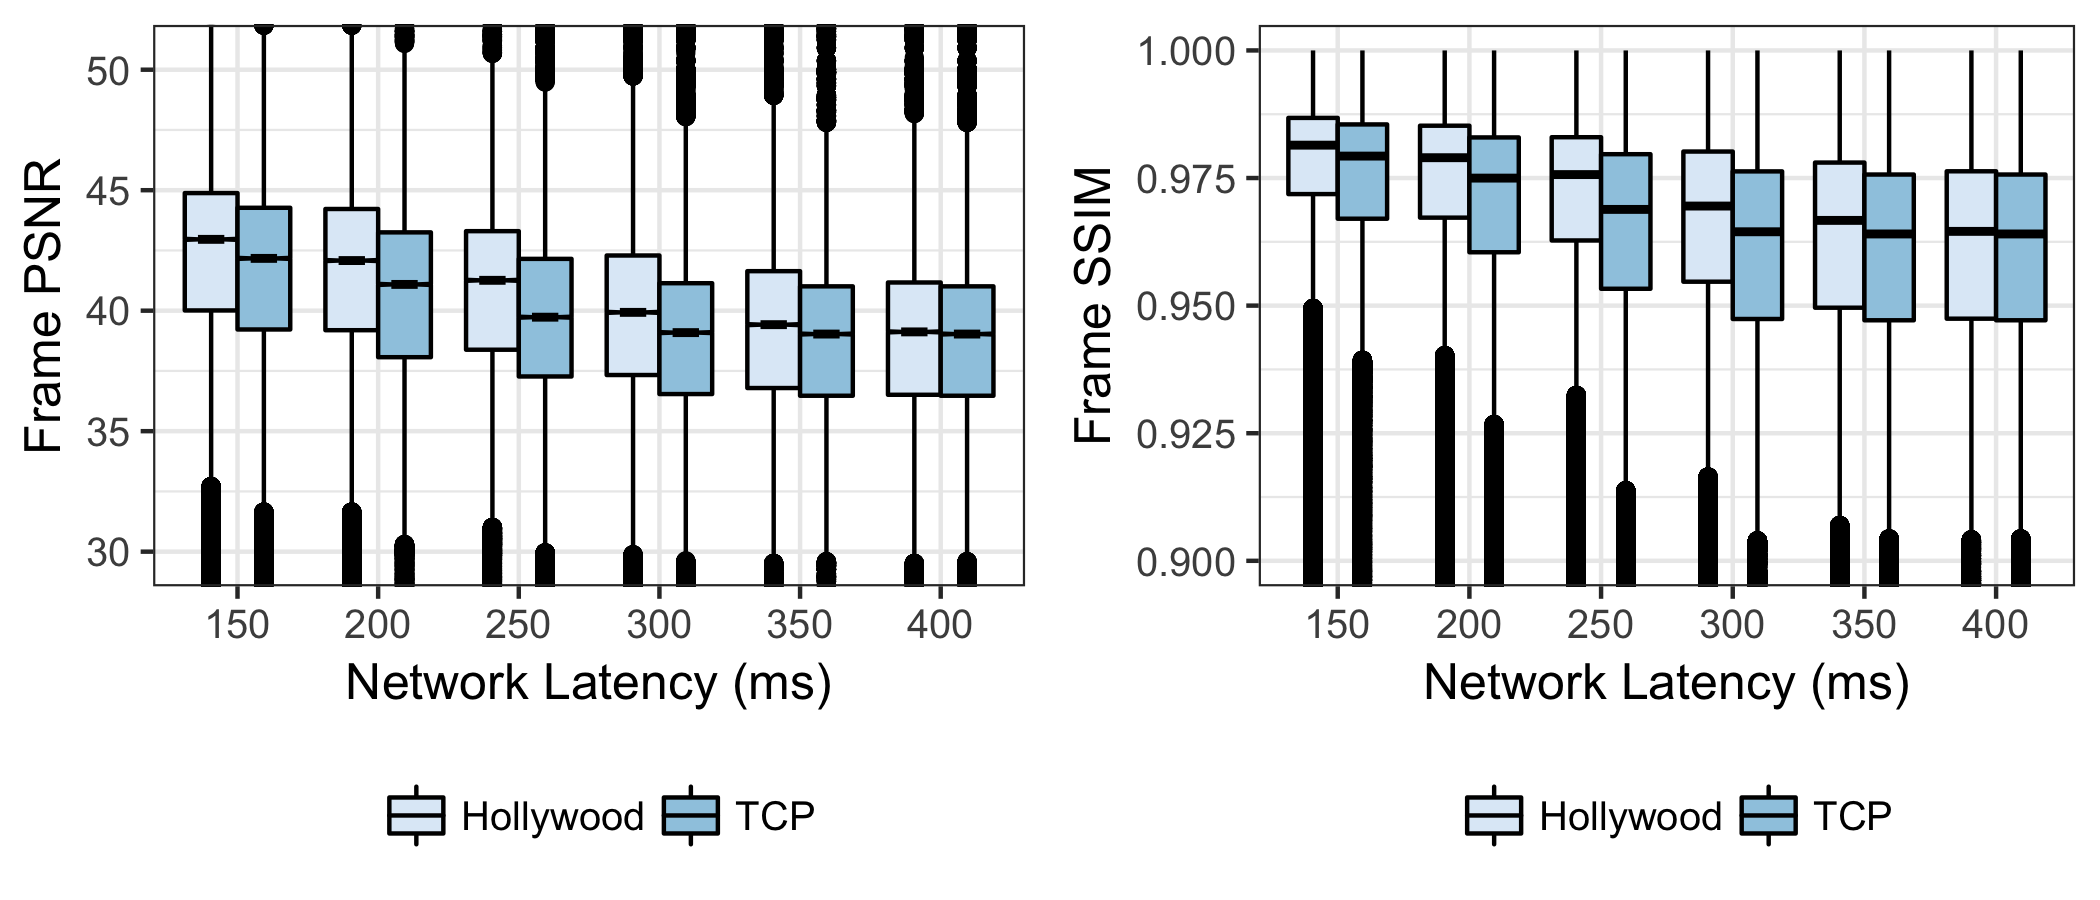
\includegraphics[width=\columnwidth]{figures/results/qoe_sn_loss_p2.png}
  \caption{Impact of delay on quality of experience. Test networks were 5Mbps with 0.2\%loss 
           with variable delay.}
  \label{fig:qoe_delay2}
\end{figure}

\begin{figure}
  \centering
  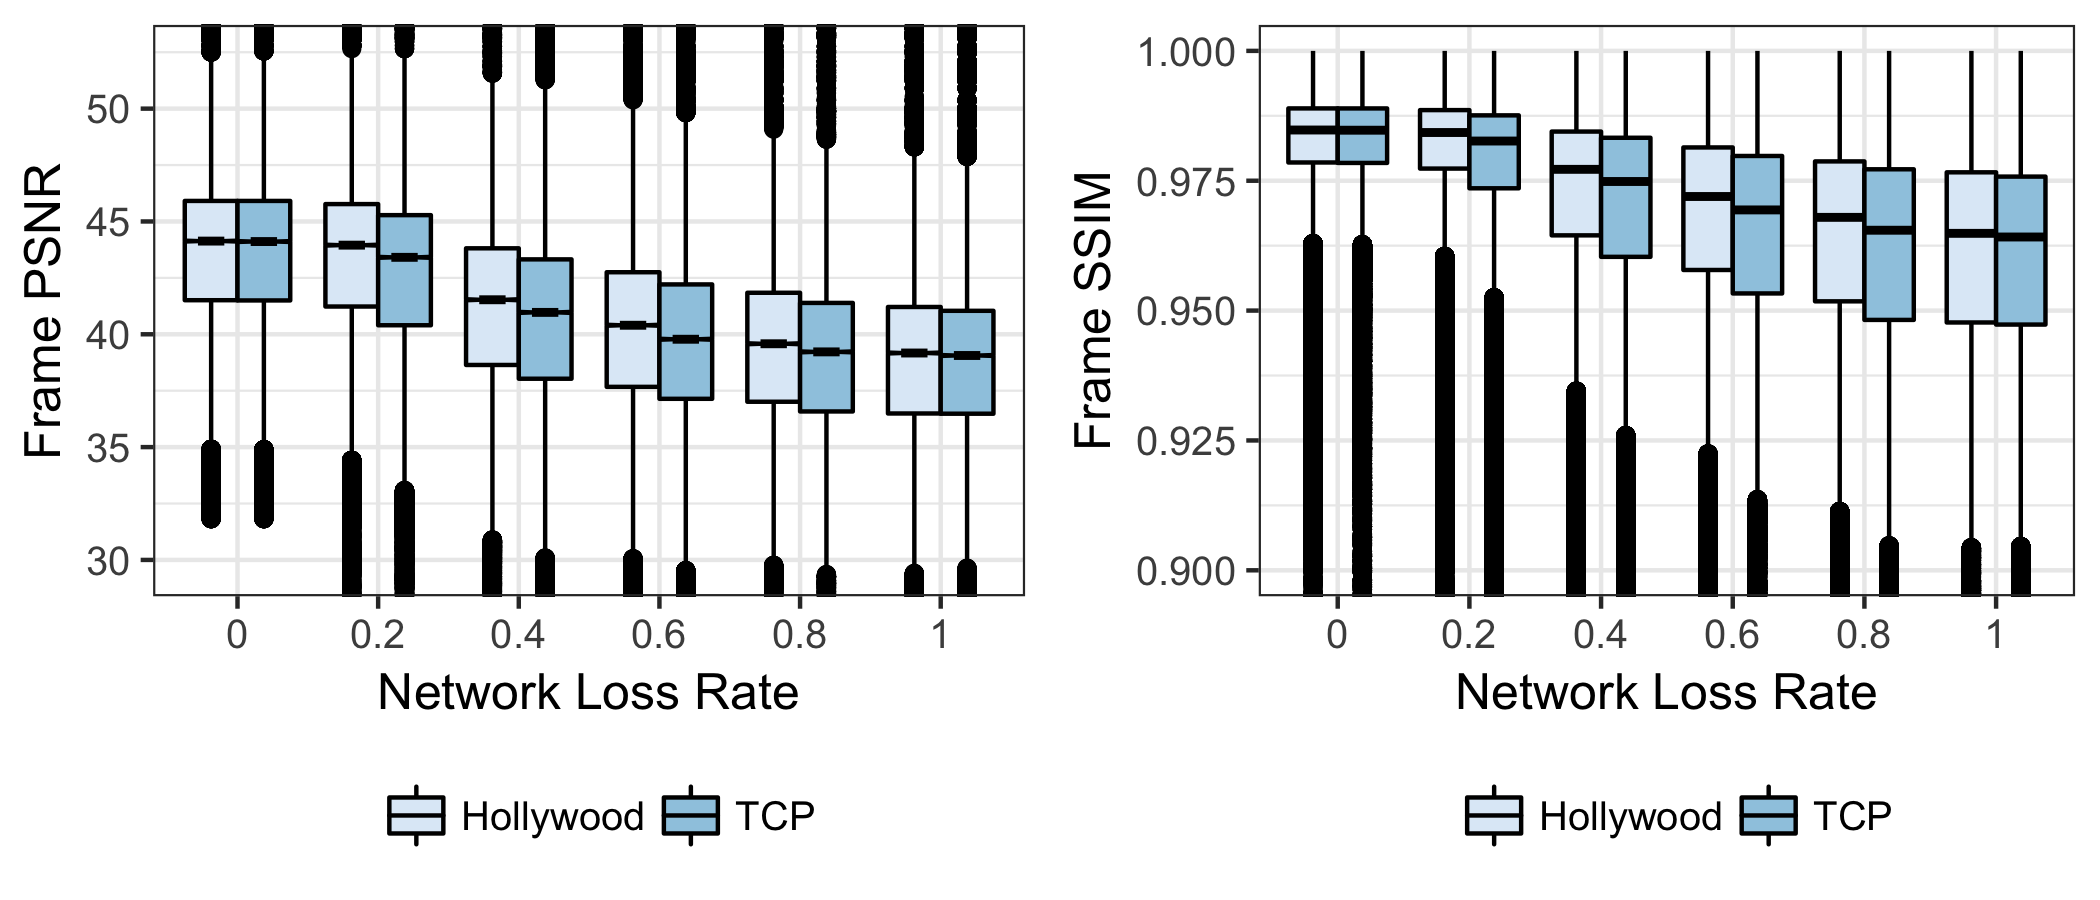
\includegraphics[width=\columnwidth]{figures/results/qoe_sn_delay_d100.png}
  \caption{Impact of packet loss on quality of experience. Test networks were 5Mbps with 100ms 
           with variable loss rates.  The TCP Hollywood-based client maintains a higher PSNR 
           and SSIM than standard TCP.}
  \label{fig:qoe_loss}
\end{figure}

\subsection{Other Testing}

We represent in this paper results from cases where the stall events were within
acceptable limits for a range of latency and loss values. However, we tested for other
conditions as well. For delay variation testing with a fixed loss rate at 0.03\%, we found
that both protocols performed equally with no stall event for delays as high as 400ms. For
a loss rate of 0.8\%, the stall duration was about 300s even at a delay of 200ms for the
standard TCP-based client. For the TCP Hollywood-based client, the stall events were reduced 
by 40\% but nearly 150
messages were discarded. Similarly, for a loss rate of 2\%, stall durations were as high as
300s when running over standard TCP with a 100ms network latency, while the use of 
TCP Hollywood reducing stall durations 
to around 230s at the cost of heavy losses. Given that such high levels of stalling will
any way be unacceptable to users, we feel that attempting to evaluate which protocol
performed better is of little consequence.

To evaluate the suitability of the adaptation algorithm in fluctuating network conditions,
we ran tests using the twelve network profiles (\emph{a} - \emph{l}) used by Spiteri et.
al.\ in their evaluation of the BOLA algorithm \cite{spiteri2016bola}. The profiles cover a
wide range of loss rates, delays and bandwidths and network conditions are changed during
the tests every 30 seconds. Since some bandwidths in the test were lower than the lowest
bit-rate in our test videos and the buffer length was limited to 16 seconds, we observed
stall events, especially for the more aggressively changing profiles (profiles \emph{g} to
\emph{l}). Generally, the use of TCP Hollywood lowered the stall events, as shown in Figure
\ref{fig:stall_profiles}. Start-up delay was similar for clients using both protocols,
although some profiles with longer network delays in the beginning benefited from the use of TCP
Hollywood. 

\begin{figure}
  \centering
  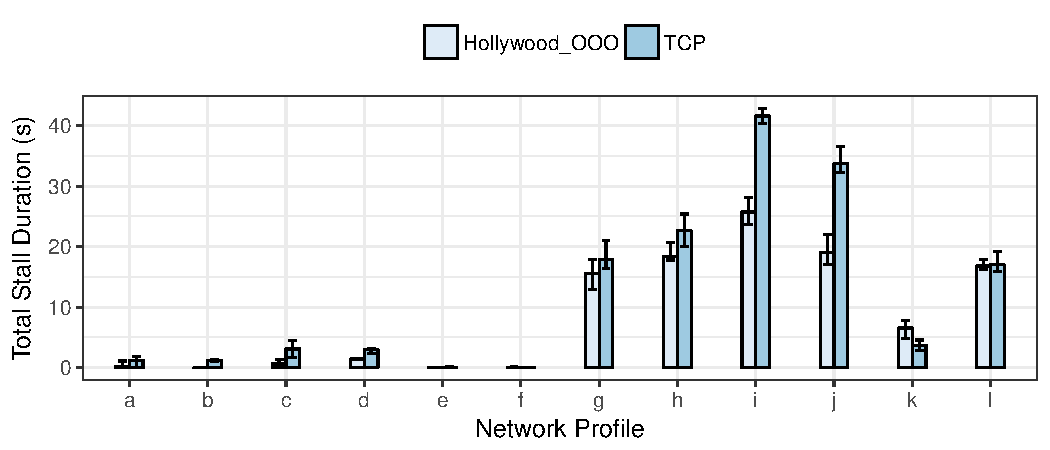
\includegraphics[width=\columnwidth]{figures/results/stall_vn_all.pdf}
  \caption{Stall events are reduced for TCP Hollywood for all except profile k, where 
           latencies are under 20 ms and bandwidth levels between 9Mbps and 1Mbps. }
  \label{fig:stall_profiles}
\end{figure}

\begin{figure}
  \centering
  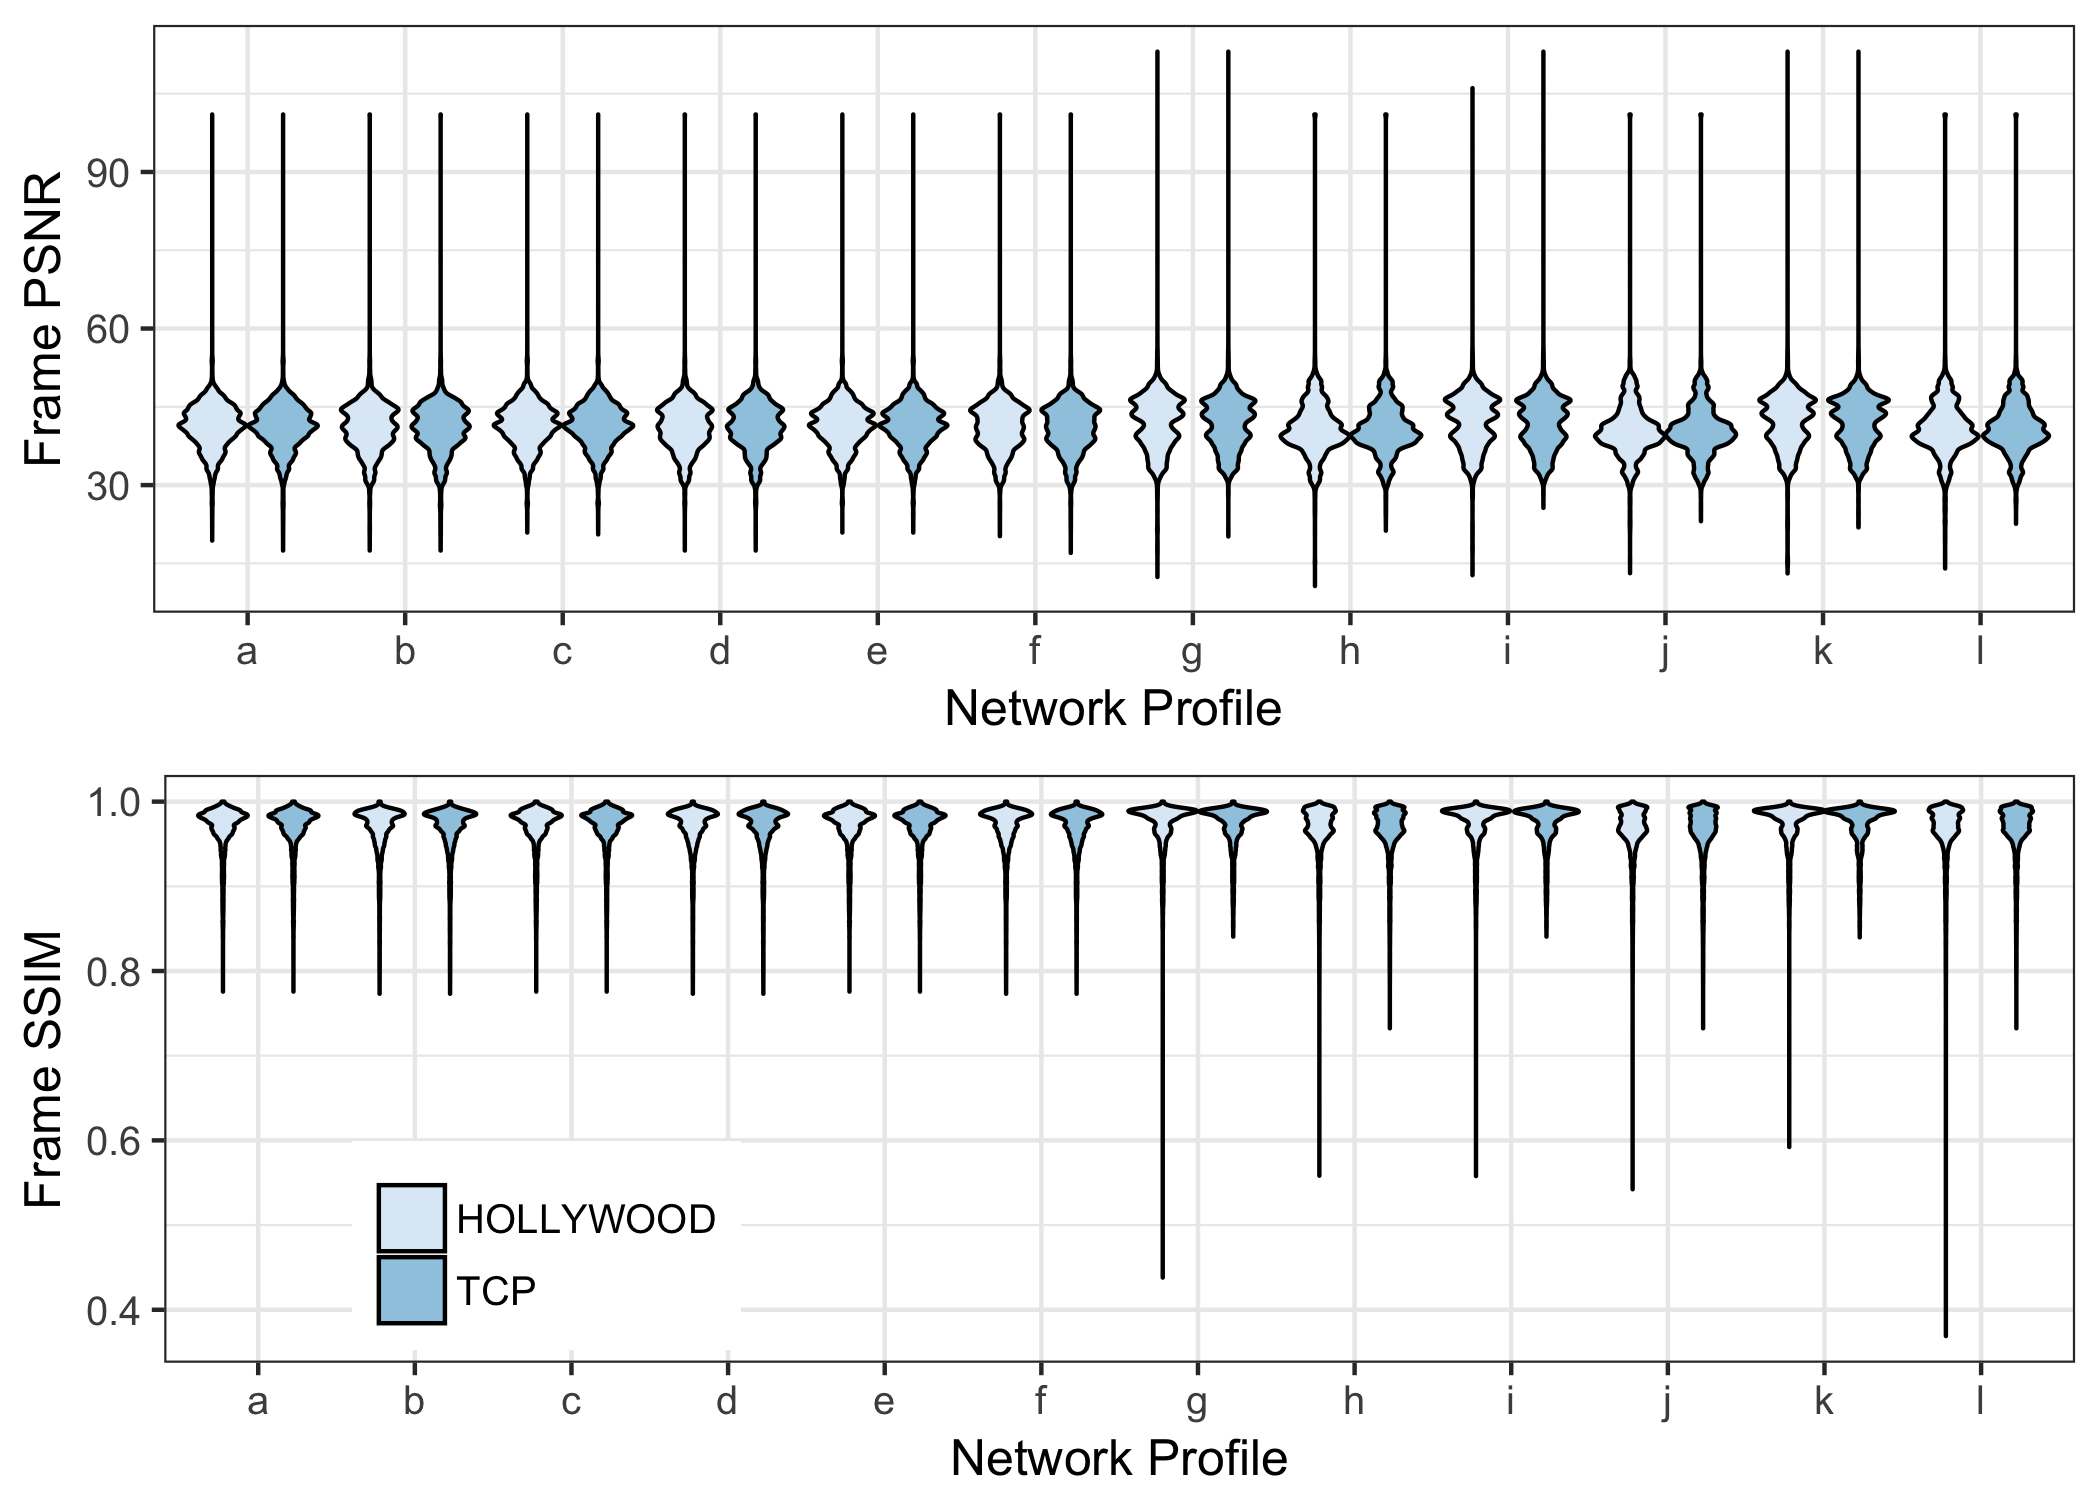
\includegraphics[width=\columnwidth]{figures/results/qoe_vn_all.png}
  \caption{Quality of experience profiles. PSNR and SSIM values of various network profiles 
           revealed similar results for both standard TCP and TCP Hollywood-based clients. The 
           shape of the violin graph reveals more information about the frequency of values, 
           showing the similarity in the download quality of both protocols with the tails in 
           SSIM plot representing the effect of lost messages.}
  \label{fig:qoe_profiles}
\end{figure}

A violin plot of the PSNR and SSIM values shows the frequency of each value in Figure 
\ref{fig:qoe_profiles}. The similarity in the shape of the plot for clients using both 
standard TCP and TCP Hollywood shows that both protocols downloaded similar quality chunks, 
as observed in the average bit-rate results. The TCP Hollywood-based client had 
a lower number of downward rate switches than the standard TCP-based client for almost all 
profiles, as shown in Figure \ref{fig:ratechange_profiles}. The client using BOLA working
with TCP Hollywood generally adapted faster to a higher bit-rate and was able to sustain a
higher bit-rate for longer than the client using standard TCP. However, this also meant that 
the TCP Hollywood client would drop suddenly to a lower rate while the standard TCP-based 
client would drop
gradually. If the degradation lasted less than the 30 seconds defined by the profiles, as
may be the case for real networks, the TCP Hollywood-based client is more likely to sustain 
the current bit-rate without dropping at all. A sample bit-rate adaptation for network profile 
\emph{g} is shown in Figure \ref{fig:adaptation_profile}. Note from Figure \ref{fig:qoe_profiles}
previously showed that the TCP Hollywood-based client does suffer from message losses in profile 
\emph{g} and future work should include exploring improvements in the adaptation algorithm to 
limit the number of discarded messages in favour of stalls in the presence of high losses. 


\begin{figure}
  \centering
  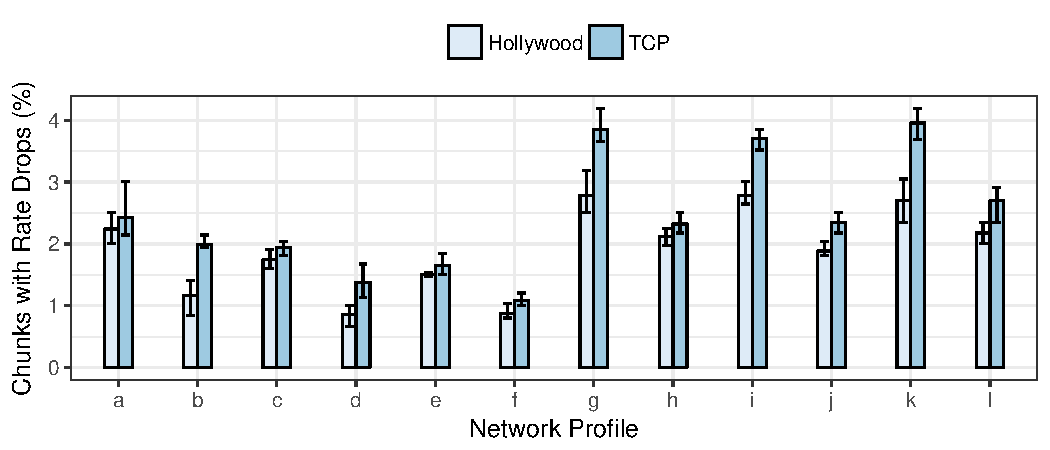
\includegraphics[width=\columnwidth]{figures/results/ratedrops_vn_all.pdf}
  \caption{Slight improvements in startup delay for all profiles is seen for TCP Hollywood. }
  \label{fig:ratechange_profiles}
\end{figure}

\begin{figure}
  \centering
  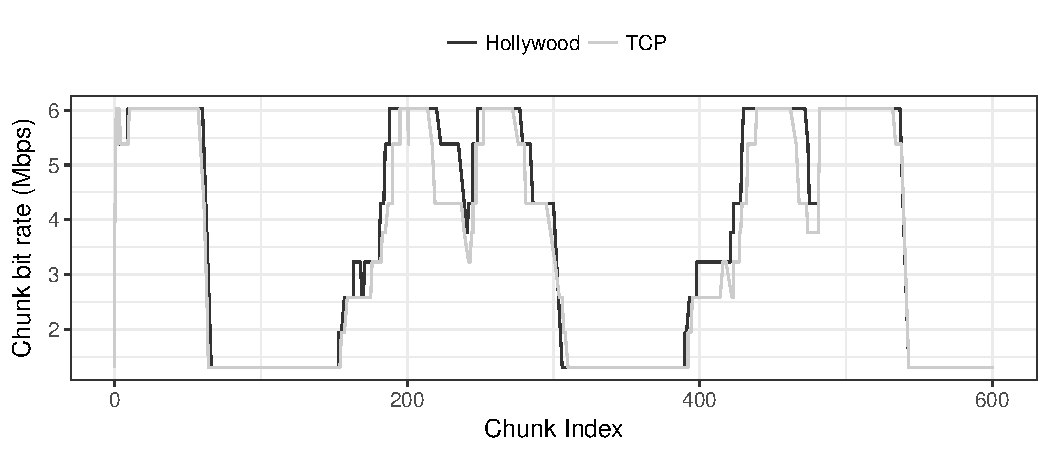
\includegraphics[width=\columnwidth]{figures/results/timeline_example_vn.pdf}
  \caption{TCP Hollywood allows the adaptation algorithm to adapt more quickly to higher bit-rates and also to sustain them for longer periods in the presence of network degradation. }
  \label{fig:adaptation_profile}
\end{figure}

\section{Related Work}
\label{sec:related}

HTTP adaptive streaming has become the de-facto standard for on-demand video streaming.
MPEG-DASH, an International Standard, is similar to other flavours of HAS, in that the
architecture involves a client requesting discrete chunks of media over HTTP, at a rate
determined by its adaptation algorithm. HAS protocols, by virtue of their use of chunked
encodings and HTTP over TCP, introduce significant latency, and rely heavily upon
buffering to maintain quality-of-experience. However, a previous study has shown that
latency, in a local network, can be reduced to as low as 240ms. The cost of this was
higher packaging overhead, with increases of up to 13\%.

An obvious application-layer approach to reducing latency in MPEG-DASH is to reduce the
size of chunks; however, doing this leads to a significant increase in the number of HTTP
requests sent. Wei and Swaminathan \cite{wei2014} propose using HTTP/2's server push
mechanism to reduce the number of requests, potentially only requiring a single HTTP
request across the entire stream. Xiao et al. \cite{xiao2016dash2m} take a similar
approach, but focus on mobile devices. While the use of HTTP/2 provides server push and
multi-streaming (and so eliminates head-of-line blocking at the application-layer), using
standard TCP means that the application will still be impacted by head-of-line blocking.
In the event of loss, data will be delayed by more than one RTT \cite{mcquistin2016tcp2};
this is problematic in low-latency applications. he use of multiple simultaneous
TCP connections provides a delivery model that is analogous to a multi-streaming protocol.
However, these connections do not share flow and congestion control state, which degrades
their performance. Further, managing these connections introduces complexity at the
application-layer.

Our approach attempts to eliminate the latency associated with head-of-line blocking by
using TCP Hollywood, whose message-oriented unordered delivery model is well suited to
low-latency applications. Other transport-layer solutions include QUIC
\cite{draft-ietf-quic-transport-latest}, a UDP-based protocol with support for stream
multiplexing. Importantly, evaluations conducted over QUIC \cite{bhat:2017:not-so-quic}
have shown that MPEG-DASH QoE is degraded. 

Neither of these approaches -- application-layer changes (e.g., using HTTP/2) or 
novel transport-layer protocols (e.g., TCP Hollywood or QUIC) -- alone is sufficient to
improve application performance. Both are required: application-layer changes are
necessary, but these must be supported by the semantics of the underlying transport
protocol. The application-layer modifications we propose here are likely to be compatible
with other multi-streaming transport-layer protocols, including QUIC.

Complementary latency-reducing approaches include a server and network-assisted variant
of MPEG-DASH, SAND \cite{thomas2015enhancing}, is also in development, and will form part
of the MPEG-DASH standard. SAND enhances MPEG-DASH with asynchronous network-to-network
and network-to-client quality-related message exchange. A Software Defined Networking
(SDN) based approach has been shown to improve user QoE by providing the client with
network performance and cache content information to assist the cache and bit-rate
selection while using the SDN network to optimise the caches \cite{bhat2017network}.
Additionally, Fr\"ommgen et al. \cite{frommgen2017programming} propose a programming model
for multipath TCP scheduling; the delivery model of TCP Hollywood, combined with the type
of traffic being carried, make this an interesting basis for future work. For example,
exposing message deadlines to a multipath scheduler may increase the proportion of
messages that meet their deadline.
\section{Conclusion}
\label{sec:conclusion}

In this work, we evaluated the effects of unordered delivery on MPEG-DASH clients, using TCP Hollywood. We
observed that by eliminating head-of-line blocking on a chunk and message level, 
an MPEG-DASH client using TCP
Hollywood is able to significantly reduce stall events while also slightly reducing start-up
delay and improving download quality. The observations and lessons learnt during the
course of this study can also be applied to other transports that support non-reliable
streams, such as SCTP and QUIC. 

\appendix
\section{Reproducibility}

To aid with reproducibility, we provide all of the source code used in generating the
results described in this paper, alongside a Makefile that describes and performs the
process of performing the experiments, processing and graphing the results, and produces
the paper. The source code for the paper is available at \url{http://researchdata.gla.ac.uk/XYZ}\footnote{\todo{Replace with institutional data repository URL for camera-ready}}.

Our evaluations require a modified Linux kernel, and each run of the evaluation simulates
different network parameters. To manage this complexity, we have split the paper's build
process into a series of stages. In this section, we describe the inputs and outputs of
each stage. We start by describing the required dependencies.

\subsection*{Dependencies}

The experiments are conducted within virtual machines, that use Linux with the TCP
Hollywood kernel extensions and API installed. VirtualBox and Vagrant are used to manage
these virtual machines. Each experiment run involves streaming Big Buck Bunny over a 
simulated network; after this, FFmpeg is used to perform SSIM and PSNR analysis between
the streamed version and a reference copy. Finally, Python and R are used to analyse and
graph the results of the experiments. The versions that were used in our testing are shown
in brackets; other versions may work.

\begin{itemize}
\item FFmpeg (3.4.2)
\item Python (2.7)
\item R (3.4.3) and packages (rkvo, ggplot2, data.table)
\item Vagrant (2.0.2)
\item VirtualBox (5.2.6r120293)
\item xz (5.2.3)
\end{itemize}

The experiments use the TCP Hollywood kernel and API. These are located in the following
repositories, and the specified versions used by the experiments:

\begin{itemize}
\item Kernel: \url{https://github.com/lumisota/tcp-hollywood-linux} \\ (version \texttt{0bb4a643})
\item API layer: \url{https://github.com/lumisota/hollywood-api-video} (version \texttt{325c415f4492d0eeebc96af87bca94826aed1d75})
\end{itemize}

These versions of the TCP Hollywood kernel and API included with the source code for the
paper, in the data repository version described above.

For readability, whenever this section refers to TCP Hollywood, it is these versions that
have been used.

Mininet\footnote{\url{http://mininet.org}} (version 2.2.1) is used to simulate the network
for each run. This is installed, and run, within the TCP Hollywood Vagrant box, and is
not required to be installed on the host machine.

\subsection*{Stage 1}

TCP Hollywood is comprised of a set of modifications to the Linux kernel, and a user-space
API layer. The first stage involves building a virtual machine image that has the TCP
Hollywood kernel. Vagrant is used for this process; a clean Ubuntu 14.04 box is downloaded,
upon which the specified version of the TCP Hollywood kernel is downloaded and installed.

\subsubsection*{Inputs}
\begin{itemize}
\item TCP Hollywood kernel
\item Ubuntu 14.04 (trusty) Vagrant base box
\end{itemize}
\subsubsection*{Outputs}
\begin{itemize}
\item TCP Hollywood kernel Vagrant box
\end{itemize}

\subsection*{Stage 2}

The next stage is to install the TCP Hollywood API within the Vagrant box. This includes
installing the modified HTTP client and server used in the experiments. In addition,
mininet is installed, for use in simulating the network required by the experiments.

\subsubsection*{Inputs}
\begin{itemize}
\item TCP Hollywood kernel Vagrant box
\item TCP Hollywood API
\end{itemize}
\subsubsection*{Outputs}
\begin{itemize}
\item TCP Hollywood Vagrant box
\end{itemize}

\subsection*{Stage 3}

The third stage involves conducting the experiments themselves, with a virtual machine
(using the TCP Hollywood Vagrant box) instantiated for each run. The experiments involve
streaming Big Buck Bunny over network, simulated using Mininet. The network conditions are specified
by network profiles (listed in the Makefile as \texttt{SN\_RUNS} and \texttt{VN\_RUNS});
these are files that describe the network conditions (e.g., bandwidth, delay, loss rates).
For each profile, the experiment is run both with TCP and TCP Hollywood, to compare the
two. Finally, to produce the graphs in this paper, each run is repeated. We use 10
repetitions by default; this can be controlled using the \texttt{RUN\_NUMBERS} variable
in the Makefile. 

Each run produces a set of files: logs from both the client and server, describing the
application-layer activity (e.g., what is sent or received); a tcpdump taken at the
server; and QoE logs (SSIM and PSNR analysis) that result from comparing the streamed
video to the reference copy.

\subsubsection*{Inputs}
\begin{itemize}
\item TCP Hollywood Vagrant box
\item Big Buck Bunny (as MPEG-DASH chunks)
\item Big Buck Bunny reference (1080p)
\item Network profiles
\end{itemize}
\subsubsection*{Outputs}

Each experiment run produces:
\begin{itemize}
\item Client logfile
\item Server logfile
\item Server tcpdump
\item SSIM logfile
\item PSNR logfile
\end{itemize}

\subsection*{Stage 4}
The previous stage produces output files for each experiment, giving application-layer
activity, and QoE data. In this stage, these output files are aggregated processed,
allowing for analysis and graphing in the next stage.

Broadly, the experiments fall into two groups: those with static network conditions, that
do not change throughout the stream, and those with variable network conditions, where
parameters, such as bandwidth and delay, are changed every 30 seconds. The results of
experiments within each group, and for each network profile, are aggregated together.

\subsubsection*{Inputs}
\begin{itemize}
\item Stage 3 output files
\item Stage 4 Python and R scripts
\end{itemize}
\subsubsection*{Outputs}

Each group (static or variable) produces (aggregated by network profile):
\begin{itemize}
\item Aggregated PSNR data
\item Aggregated SSIM data
\item Aggregated QoS data (e.g., rebuffering events)
\item Aggregated bitrate data
\end{itemize}

\subsection*{Stage 5}
In this stage, the processed results files generated by the previous stage are graphed.
\begin{itemize}
\item Stage 4 output files
\item Stage 5 R scripts
\end{itemize}
\subsubsection*{Outputs}

\begin{itemize}
\item Figures 3 to 16 inclusive
\end{itemize}

\subsection*{Stage 6}
With the results of the experiments graphed, the final stage is to build the paper.

\begin{itemize}
\item Paper TeX and BibTeX files
\item Figures (static and those generated in stage 5)
\end{itemize}
\subsubsection*{Outputs}
\begin{itemize}
\item Paper
\end{itemize}

\subsection*{Discussion}

The source code that we have made available, alongside this appendix, should be sufficient
for repeating the experiments conducted in this paper. However, making the paper
reproducibility introduces a number of challenges, and encounters various limitations. We
discuss and reflect on those in this section.

Each evaluation run makes use of a simulated network. As part of this simulation, random
packet loss is introduced. As this is non-deterministic, the results generated by
building the paper will be different between different builds, including the published
work. Making repetitions not only allows us to determine the statistical significance
of the results we see, but also ensures that the paper discusses general trends that hold
true between builds. However, where we discuss a particular run (e.g., in Section
\ref{sec:other_testing}), it is inevitable that the text will not match results generated
in other builds. It is not clear how such non-determinism should be handled when
considering reproducibility: while the general trends, and therefore the conclusion of the
paper, hold, a given run will be different.

Our particular testing requirements (i.e., a modified Linux kernel) lends itself to using
virtual machines, and orchestrating those machines programmatically (e.g., by using
Vagrant). This minimises the dependencies that need to be installed on the host machine:
for example, each run uses Mininet, but this runs within the virtual machine, rather than
on the host machine. However, this methodology also introduces limitations: our
evaluations essentially depend on a particular Linux environment, and packaging this for
reproducibility is non-trivial. While including the TCP Hollywood kernel and API code
goes some way towards preventing decay in the reproducibility of the paper, some
dependencies on external sources remain. For example, several software packages are
installed using package managers; this relies upon the availability of the underlying
repositories. There exists a trade-off between how long the paper can be usefully
reproduced using the assets we provide, and the tractability of determining and including
\emph{all} of the dependencies that exist. Understanding this trade-off and making
appropriate choices is important if reproducibility is to be improved more generally.

\bibliographystyle{ACM-Reference-Format}
\bibliography{dash_hollywood}

\end{document}
